\documentclass[11pt, A4paper, english]{article}
\usepackage{amsfonts}
\usepackage{amsmath}
\usepackage{amssymb}
\usepackage{amsthm}
\usepackage{babel}
\usepackage{cite}
\usepackage{color}
\usepackage{float}
\usepackage[T1]{fontenc}
\usepackage{graphicx}
\usepackage[colorlinks]{hyperref}
\usepackage[utf8]{inputenc}
\usepackage{listings}
\usepackage{textcomp}
\usepackage[numbib,nottoc]{tocbibind}


\definecolor{dkgreen}{rgb}{0, 0.6, 0}
\definecolor{gray}{rgb}{0.5, 0.5, 0.5}
\definecolor{daynineyellow}{rgb}{1.0, 0.655, 0.102}
\definecolor{url}{rgb}{0.1, 0.1, 0.4}

\lstset{frame=tb,
	language=Python,
	aboveskip=3mm,
	belowskip=3mm,
	showstringspaces=false,
	columns=flexible,
	basicstyle={\small\ttfamily},
	numbers=none,
	numberstyle=\tiny\color{gray},
	keywordstyle=\color{blue},
	commentstyle=\color{daynineyellow},
	stringstyle=\color{dkgreen},
	breaklines=true,
	breakatwhitespace=true,
	tabsize=3
}

\lstset{inputpath="C:/Users/Torstein/Documents/USN/IIA2017"}
\graphicspath{{C:/Users/Torstein/Documents/USN/IIA2017/Assignment 1/}}
\hypersetup{colorlinks, urlcolor=url}

\author{Torstein Solheim Ølberg}
\title{Pokémon Kanto Starter Quiz Game}



%\lstinputlisting{Filnavn! type kodefil}
%\includegraphics[width=12.6cm, height=8cm]{Filnavn! type png}



\begin{document}
	\maketitle
	\clearpage

	\section{Introduction}
For a long time I have found lots of quiz pages on the internet, all of them some sort of quiz where you have to guess names for something. Either its the name of the Pokémon in the different generations, or its the 100 most mentioned characters in some book series. The problem with all these quiz pages is that they give you a timer you have to finish within or you automatically lose. This is much less ideal for someone whom simply wants to know how fast they can do it. For this reason, I have created a simple program testing the concept of creating this in LabVIEW \cite{LabView}. I have limited the program to only the first 9 Pokémon and a simple timer counting up.

	\section{Implementation}
The program needs a loop continuing until a stop button is pushed or the game is finished and the player has won. In the front panel the program needs a timer which is updated inside the loop and counts the seconds, minutes and hours having elapsed since start. I have chosen three numerical indicators to show the seconds, minutes and hours separately. Then the program needs a display where the correct names will appear when they are guessed and an input window where the player can give their guesses. These need to be updated in the while loop as well. I chose to use a table for the display window and a string control for the input window. Finally, there is a need for a string indicator to give feedback to the user during the game, which also must be updated in the while loop. \\

To handle the updating of the different things inside the loop, I chose to use a case structure with three cases and a shift register. The initialisation case where the start of the game is set up, the event handler which handles any changes, and the stop case which is called to stop the program. In the event handler I include an event structure. This event structure has a timeout of ten milliseconds and needs to take care of two events. First it needs to stop the program if the stop button is pushed. This is done by sending a stop string to the shift register with the name of the stop case. The second event is when a key is pressed in the input window. To handle this event the code must first check which key is pressed, and if it is enter, the focus from the window most be removed. Then the input must be checked if it is correct and the display table, and feed back string indicator, must be updated. Then a counter of how many guesses have been made correctly must be incremented by one. And finally the input window must be cleared and refocused, also only if enter was the key that was pressed. To ensure these events happen in the order specified above, they are encased in a flat sequence structure. \\

The key press check and the test for if the guess is correct are split of into two separate subVIs. The key that is pressed is checked by finding its index in an array containing the keys enter and return. If the index is 0 or above, the pressed key is enter and a greater than or equal to zero returns True. Else the index checker returns minus one and the greater than or equal to zero returns False. The guess checker takes the guess and the state of the display table as input. Check if the guess is in an answer array, checks if the guess is not already in the display table, creates a new display table with the guess if it is correct and returns this and a boolean of whether the guess was true or not.

The shift register must be updated during each case in the loop. For almost all cases, the string given is simply the name of the event handler case again, but if the stop button is pushed or the number of correct guesses reaches the total amount of names included, the string must be the name of the stop case. \\

Finally, the seconds, minutes and hours must be handled in a flat sequence structure outside the case structure but inside the while loop. First the seconds are calculated by use of the High Resolution Relative Seconds Vi. The number of seconds are calculated from equation \ref{eq:1}
		\begin{equation}
s_{\text{since start}} = s_{\text{now}} - s_{\text{at start of program}}
\label{eq:1}
		\end{equation}
where the variables at the right hand side are the machine seconds at the start of the program and now. When the seconds reach 60, the value of the variable saving the machine seconds at the start of the program must be reset to that instants value, and the number of minutes must be incremented by one. Finally, when the number of minutes reach 60, they must be reset to zero and the hour counter must be incremented by one.
	\section{Results}
The program can be viewed or downloaded from my GitHub page \cite{github_repo}. You can also see an image of the program as a player would see it, during a run, in figure \ref{front_panel}.
		\begin{figure}
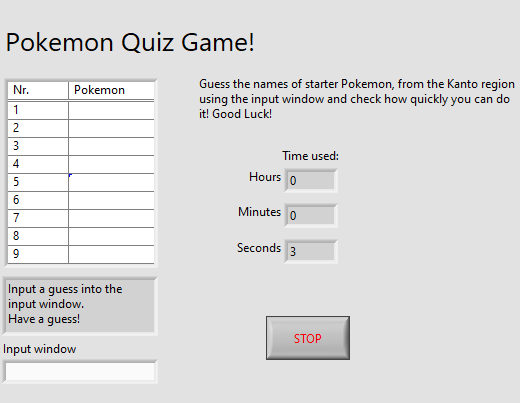
\includegraphics[width=12.6cm, height=8cm]{screenshot_front_panel.png}
\caption{Image of the front panel of the program during execution. You can see the display table, feedback window, input window, timer and stop button.}
\label{front_panel}
		\end{figure}

	\section{Discussion}
The program is a executable and performs the task i set out to do. However, there are a number problems with it that can be improved upon. First of all, the program is limited to only 9 pre specified names at the moment. This could be improved by adding more names to the answer array. However, an even better way to do this would be to either import the answers from a local file or download a list of the names from a web page. This would be much easier to update later and it would be possible to add different categories as well without everything having to be stored in active memory even when its not used. \\

For now you also have to write down or simply remember the time you use yourself. A better solution would be to include a scoreboard stored in a local file that is updated on victory. This would also better help a player compare their score if they play with different categories and allow for easier comparing between different players. \\

Furthermore, the game now starts as soon as the program is started. This is not ideal for new players, as they would need to use time in the beginning to read what they want to do and how they are to play. This can be fixed by adding a start button, which the player presses to start the program. An even better solution is to add a menu where the program is explained in the beginning, where a start button is included. This would combine well with the score board and the ability to chose different categories. These could be different pages viewed by selecting different buttons. \\

Another improvement would be to add the choice of other languages to the game, as it now only is in English. A drop down menu of other languages would be useful, and would combine well with a menu before the game.

	\section{Conclusion}
I have used the software LabView to develop a quiz game where the player needs to guess the names of the nine starter Pokémon from the Kanto region. The program includes a display, an input window, a feedback window, a timer, and a stop button, which are all controlled and updated in a while loop. The program works according to the goals and restrictions I applied, but it would be very useful to add different improvements to it. especially, adding the ability import the answers from a file outside the program and a menu to control when you start and with which settings would be ideal.

		\begin{thebibliography}{9}
			\bibitem{LabView}
National Instruments Corp.; \\
LabView [Webpage]; \\
Available at: \url{https://www.ni.com/en-no/shop/product/labview.html}
			\bibitem{github_repo}
T. S. Ølberg; \\
GitHub repository of code for Assignment 1 [Webpage]; \\
Available at: \url{https://github.com/MrTorstein/IIA2017/tree/main/Assignment\%201s} \\
Published 14/01-2023
%			\bibitem{Name of referance!}
%Name of Author, Name of Author, ...!; \\
%Title of article!, Pages used! \\
%Year of release!, Town published!: Publisher! \\
		\end{thebibliography}
\end{document}